\documentclass[letterpaper,10pt]{article}

\usepackage{tikz}
\usepackage{caption}

\setlength{\headheight}{0in}
\setlength{\marginparsep}{0in}
\setlength{\footskip}{0in}
\setlength{\headsep}{0in}
\setlength{\marginparwidth}{0in}
\setlength{\marginparpush}{0in}
\setlength{\voffset}{0in}
\setlength{\hoffset}{-1in}
\setlength{\voffset}{-1in}
\setlength{\oddsidemargin}{0.75in}
\setlength{\evensidemargin}{0.75in}
\setlength{\topmargin}{0.75in}
\setlength{\textheight}{9.5in}
\setlength{\textwidth}{7in}
\setlength{\parindent}{0in}
\setlength{\parskip}{10pt} %change this to match font size

\pagestyle{empty}
\definecolor{gray}{gray}{0.75}
\usetikzlibrary{shapes,arrows,calc}

% define block styles
\tikzstyle{line} = [draw, -latex']
\tikzstyle{block} = [draw, rectangle, text centered, minimum height=2em]
\tikzstyle{mlblock} = [draw, rectangle, text width=10em, text centered, minimum height=2em]
\tikzstyle{decision} = [draw, diamond, text width=4.5em, text centered, node distance=3cm, inner sep=0pt]
\tikzstyle{cloud} = [draw, rectangle, text centered, rounded corners, minimum height=2em]

\begin{document}
    Albert Chang and Nipun Chopra\\
    CSE-380 A6\\
    University at Buffalo\\
    Dr. Kris Schindler\\
    April 26, 2011\\
    \textit{Lab 7 Documentation}

    The objective of Lab 7 was to recreate the classic Donkey Kong arcade game.
    In this game, the princess, whom was captured, needs to be saved. This is
    accomplished by dodging barrels on the way to the top of the map. Mario moves
    left or right freely, and jump anytime he is walking on a floor. He cannot
    jump off a ladder. Jumping action must be shown. Mario dies either when he
    collides with a barrel or falls from a floor. If Mario jumps over a barrel,
    five times the current level of the game is awarded. The only other time
    points are awarded is when Mario reaches the princess, then 100 times the
    current level is awarded. Every 1000 points, a life is gained. The barrels
    roll from top to bottom and has a 50\% chance of falling down any ladder it
    comes across.

    For the interface, the classic WASD game keys were used to control Mario.
    The serial port handled outputting as well as accepting key-presses. The
    LEDs indicated the amount of lives left. The seven-segment display
    indicated which level the player is on. The other input was from the
    momentary push button, which pauses the game. The map was already provided
    for us as such:

    \begin{center}
        \begin{minipage}{30mm}
\begin{verbatim}
   SCORE:00000  
+--------------+
|              |
|   !          |
|   ===H       |
|      H       |
|&@    H       |
|-------#---H  |
|           H  |
|           H  |
|  ==H=========|
|    H         |
|    H         |
|-#--------H-  |
|          H   |
|          H   |
|  H===========|
|  H           |
|  H           |
|-----------H  |
|           H  |
|$          H  |
+==============+
\end{verbatim}
        \end{minipage}
    \captionof{figure}{Donkey Kong Map.}
    \end{center}

    Several helper routines were created to help organize the code since it
    was a relatively complex program. When idling, the program is in an
    infinite loop in the \textit{game} routine, which is called by the C
    wrapper. Unlike the previous labs where an infinite loop outside our
    control, a recursive branching instruction in \textit{Startup.s}, this 
    infinite loop needed to have a break condition. The break conditions are
    either when the map needs to be reset or when game over is reached. The map
    is reset when either a new level is reached or when Mario loses a life.
    Game over is reached when either all levels have been completed or when all
    lives have expired. Besides that, all the \textit{game} routine does is
    set up all interfaces. Figs. \ref{flo:game 1} and \ref{flo:game 2} show
    the flowchart of the \textit{game} routine.

    \begin{minipage}{\linewidth}
        \begin{center}
    \begin{tikzpicture}[node distance=1.5cm, auto]
        \node[cloud] (origin) {Start};
        \node[block, below of=origin] (rtc) {Start RTC};
        \node[block, below of=rtc] (uart) {Initialize UART0};
        \node[block, below of=uart] (interrupts) {Initialize interrupts};
        \node[block, below of=interrupts] (timers) {Setup timer increments};
        \node[block, below of=timers] (gpio) {Setup GPIO for LEDs, 7-segment display, and push button};
        \node[block, below of=gpio] (dec) {Increase barrel ejection frequency and speed};
        \node[block, below of=dec] (clear) {Clear Map of barrels};
        \node[block, below of=clear] (first) {Eject first barrel};
        \node[block, below of=first] (mario) {Reset Mario's position};
        \node[block, below of=mario] (display) {Show initial display};
        \node[block, below of=display] (startt) {Start timers};
        \node[block, below of=startt] (lives) {Show remaining lives};
        \node[block, below of=lives] (level) {Show current level};
        \path[line] (origin) -- (rtc);
        \path[line] (rtc) -- (uart);
        \path[line] (uart) -- (interrupts);
        \path[line] (interrupts) -- (timers);
        \path[line] (timers) -- (gpio);
        \path[line] (gpio) -- (dec);
        \path[line] (dec) -- (clear);
        \path[line] (clear) -- (first);
        \path[line] (first) -- (mario);
        \path[line] (mario) -- (display);
        \path[line] (display) -- (startt);
        \path[line] (startt) -- (lives);
        \path[line] (lives) -- (level);
        \path[line, dashed] (level) -- +(0,-1.5);
        \draw[dashed] (level) +(5,-1.5) -- +(5,0);
        \path[line] (level) +(5,0) |- (dec);`
    \end{tikzpicture}
\end{center}

        \captionof{figure}{Flowchart of \textit{game} routine.}
        \label{flo:game 1}
    \end{minipage}

    \begin{minipage}{\linewidth}
        \begin{center}
    \begin{tikzpicture}[node distance=1.5cm, auto]
        \node[decision, below of=level] (win) {Has all levels been completed?};
        \node[decision, below of=win, node distance=4cm] (lose) {Does Mario have any lives left?};
        \node[decision, below of=lose, node distance=4cm] (new) {Has a level been completed?};
        \node[decision, below of=new, node distance=4cm] (death) {Did Mario lose a life?};
        \node[block, below of=death, node distance=4cm] (gameover) {Show game over screen};
        \node[block, below of=gameover] (off) {Disable all interrupts};
        \node[cloud, below of=off] (stop) {Stop};
        \path[line, dashed] (win) +(0,2.5) -- (win);
        \path[line] (win) -- node[near start] {no} (lose);
        \path[line] (lose) -- node[near start] {yes} (new);
        \path[line] (new) -- node[near start] {no} (death);
        \path[line] (win) -| node[near start] {yes} +(-5,-16) -- (gameover);
        \draw (lose) -- node[near start] {no} +(-5,0);
        \draw (win) +(5,0) |- node[near end] {yes} (death);
        \path[line, dashed] (win) +(5,0) -- +(5,2.5);
        \draw (new) -- node[near start] {yes} +(3,0);
        \path[line] (gameover) -- (off);
        \path[line] (off) -- (stop);
        \path[line] (death) -- node[near start] {no} +(0,-2.5) -| +(3,12) -- (win);
    \end{tikzpicture}
\end{center}

        \captionof{figure}{Flowchart of \textit{game} routine, continued.}
        \label{flo:game 2}
    \end{minipage}

    The \textit{interrupt\_init} routine simply enables and classifies TIMER0,
    TIMER1, UART0, and EINT1 as fast interrupts. Fig. \ref{flo:interrupt_init}
    shows how the routine works.

    \begin{figure}[hp]
        \begin{center}
    \begin{tikzpicture}[node distance=1.5cm, auto]
        \node[cloud] (origin) {Start};
        \node[block, below of=origin] (fiq) {Classify as FIQs};
        \node[block, below of=fiq] (enable) {Enable UART0, TIMER0, TIMER1, and EINT1 interrupts};
        \node[block, below of=enable] (uart) {UART0 interrupt on RX};
        \node[block, below of=uart] (timers) {Setup TIMER interrupts};
        \node[block, below of=timers] (eint) {EINT1 interrupts on edge};
        \node[block, below of=eint] (cpsr) {Enable fast interrupts on CPSR};
        \node[cloud, below of=cpsr] (stop) {Stop};
        \path[line] (origin) -- (fiq);
        \path[line] (fiq) -- (enable);
        \path[line] (enable) -- (uart);
        \path[line] (uart) -- (timers);
        \path[line] (timers) -- (eint);
        \path[line] (eint) -- (cpsr);
        \path[line] (cpsr) -- (stop);
    \end{tikzpicture}
\end{center}

        \caption{Flowchart of \textit{interrupt\_init} routine.}
        \label{flo:interrupt_init}
    \end{figure}

    The \textit{FIQ\_Handler} is the backbone of the program. It is the routine
    which really makes the entire program work. By itself it doesn't do anything,
    but it acts as a hub, connecting interrupts with their proper routines. Fig.
    \ref{flo:fiq_handler} shows how the program works.

    \begin{figure}[hp]
        \begin{center}
    \begin{tikzpicture}[node distance=1.5cm, auto]
        \node[cloud] (origin) {Start};
        \node[decision, below of=origin] (timer) {Was the interrupt caused by the timer?};
        \node[block, below of=timer, node distance=3cm] (clear) {Clear interrupt};
        \node[block, below of=clear] (fixed) {Clear terminal and output prompt and top of box};
        \node[block, below of=fixed] (get) {Get position and direction};
        \node[block, below of=get] (updatep) {Update position and change direction if necessary};
        \node[block, below of=updatep] (updatet) {Update terminal output};
        \node[block, below of=updatet] (save) {Save positition and direction};
        \node[block, below of=save] (reset) {Reset TCR and re-enable clock};
        \node[decision, below of=reset] (uart) {Was the interrupt caused by UART?};
        \node[block, below of=uart, node distance=3cm] (input) {Read input};
        \node[block, below of=input] (set) {Adjust speed and direction based on input};
        \node[cloud, below of=set] (stop) {Stop};
        \path[line] (origin) -- (timer);
        \path[line] (timer) -- node [near start] {yes} (clear);
        \path[line] (clear) -- (fixed);
        \path[line] (fixed) -- (get);
        \path[line] (get) -- (updatep);
        \path[line] (updatep) -- (updatet);
        \path[line] (updatet) -- (save);
        \path[line] (save) -- (reset);
        \path[line] (reset) -- (uart);
        \path[line] (uart) -- node [near start] {yes} (input);
        \path[line] (input) -- (set);
        \path[line] (set) -- (stop);
        \path[line] (timer) -| node [near start] {no} +(6,-21) -- (stop);
        \draw (uart) -- node [near start] {no} +(6,0);
    \end{tikzpicture}
\end{center}

        \caption{Flowchart of \textit{FIQ\_Handler} routine.}
        \label{flo:fiq_handler}
    \end{figure}

    One of the big routine is \textit{mv\_barrel}, which goes through all the
    barrels, and updates them. Each barrel takes 32 bits to store, but only 19
    bits are actually used. Bits 0--3 store the x-position, bits 4--8 store
    the y-position, bits 9--10 store the direction, and bits 11--18 store the
    character it replaced on the map. Pathing is determined directly from
    the context information. In situations where it could fall, and the randomizer
    selects it to fall, it provides the same context as a guaranteed fall
    condition (no support under barrel). It sets a fall flag, which is used to
    change direction when the barrel lands (has support again). A barrel is
    deleted when it is at the end of the map. Refer to fig. \ref{flo:mv_barrels}.

    \begin{figure}[hp]
        \begin{center}
    \begin{tikzpicture}[node distance=1.5cm, auto]
        \node[cloud] (origin) {Start};
        \node[decision, below of=origin] (cntr) {6th barrel?};
        \node[cloud, right of=cntr, node distance=5cm] (stop) {Stop};
        \node[block, below of=cntr, node distance=3cm] (parse) {Parse position};
        \node[block, below of=parse] (restore) {Restore previous character};
        \node[block, below of=restore] (context) {Contextualize the barrel};
        \node[block, below of=context] (pathing) {Determine next move};
        \node[decision, below of=pathing] (collision0) {Is replacement character Mario?};
        \node[block, right of=collision0, node distance=5cm] (die0) {Lose a life};
        \node[block, below of=collision0, node distance=3cm] (update) {Move barrel};
        \node[decision, below of=update] (collision1) {Is the new position Mario?};
        \node[block, below of=collision1, node distance=3cm] (next) {Get next barrel};
        \path[line] (origin) -- (cntr);
        \path[line] (cntr) -- node[near start] {no} (parse);
        \path[line] (cntr) -- node[near start] {yes} (stop);
        \path[line] (parse) -- (restore);
        \path[line] (restore) -- (context);
        \path[line] (context) -- (pathing);
        \path[line] (pathing) -- (collision0);
        \path[line] (collision0) -- node[near start] {yes} (die0);
        \path[line] (die0) -- (stop);
        \path[line] (collision0) -- node[near start] {no} (update);
        \path[line] (update) -- (collision1);
        \path[line] (collision1) -| node[near start] {yes} (die0);
        \path[line] (collision1) -- node[near start] {no} (next);
|       \path[line] (next) -- +(-3,0) |- (cntr);
    \end{tikzpicture}
\end{center}

        \caption{Flowchart of \textit{mv\_barrels} routine.}
        \label{flo:mv_barrels}
    \end{figure}

    The \textit{mk\_barrel} is a straight forward routine to generate a new
    barrel. Since new barrels always have the same starting data, it is hard
    coded. Refer to fig. \ref{flo:mk_barrel}.

    \begin{figure}[hp]
        \begin{center}
    \begin{tikzpicture}[node distance=1.5cm, auto]
        \node[cloud] (origin) {Start};
        \node[mlblock, below of=origin] (ram) {Seek first available space in RAM allocated to the barrels};
        \node[block, below of=ram, node distance=2cm] (create) {Add barrel in RAM};
        \node[block, below of=create] (draw) {Update display buffer};
        \node[cloud, below of=draw] (stop) {Stop};
        \path[line] (origin) -- (ram);
        \path[line] (ram) -- (create);
        \path[line] (create) -- (draw);
        \path[line] (draw) -- (stop);
    \end{tikzpicture}
\end{center}

        \caption{Flowchart of \textit{mk\_barrel} routine.}
        \label{flo:mk_barrel}
    \end{figure}

    The \textit{rm\_barrels} routine is a little bit more involved than the
    \textit{mk\_barrel}. This routine deletes all barrels on the map. Refer to
    fig. \ref{flo:rm_barrels}. This routine uses a smart replace algorithm, when
    replacing the previous character. The only difference is that since Mario
    and a barrel can occupy the same place, a blacklist of characters is kept
    so only the original map is restored.

    \begin{figure}[hp]
        \begin{center}
    \begin{tikzpicture}[node distance=1.5cm, auto]
        \node[cloud] (origin) {Start};
        \node[decision, below of=origin] (all) {6th barrel?};
        \node[cloud, right of=all, node distance=5cm] (stop) {Stop};
        \node[block, below of=all, node distance=3cm] (parse) {Parse position};
        \node[block, below of=parse] (restore) {Restore previous character};
        \node[block, below of=restore] (del) {Delete barrel from RAM};
        \node[block, below of=del] (next) {Fetch next barrel};
        \path[line] (origin) -- (all);
        \path[line] (all) -- node[near start] {yes} (stop);
        \path[line] (all) -- node[near start] {no} (parse);
        \path[line] (parse) -- (restore);
        \path[line] (restore) -- (del);
        \path[line] (del) -- (next);
        \path[line] (next) -- +(-3,0) |- (all);
    \end{tikzpicture}
\end{center}

        \caption{Flowchart of \textit{rm\_barrels} routine.}
        \label{flo:rm_barrels}
    \end{figure}

    The \textit{mv\_mario} routine is another very involved routine. A move is 
    only made if the contextualizer allows a particular move. Mario also takes
    up 32 bits of RAM. However, he actually only needs 18 bits. Bits 0--3 store
    the x-position, bits4--8 store the y-position, bit 9 stores whether he
    jumped or not, and bits 10--17 is the character he replaced on the map.
    Figs. \ref{flo:mv_mario_1} and \ref{flo:mv_mario_2} show how the methods
    work.

    \begin{minipage}{\linewidth}
        \begin{center}
    \begin{tikzpicture}[node distance=1.5cm, auto]
        \node[cloud] (origin) {Start};
        \node[block, below of=origin] (read) {Get keyboard input};
        \node[block, below of=read] (parse) {Parse position};
        \node[decision, below of=parse] (movable) {Can Mario move?};
        \node[cloud, right of=movable, node distance=7cm] (stop) {Stop};
        \node[block, below of=movable, node distance=3cm] (mid) {Is Mario mid-jump?};
        \node[block, below of=mid] (context) {Contextualize};
        \node[decision, below of=context] (match) {valid move based on context?};
        \node[block, below of=match, node distance=3cm] (restore) {Restore previous character};
        \node[block, below of=restore] (move) {Move Mario};
        \node[block, below of=move] (save) {Save previous character};
        \node[block, below of=save] (update) {Update output buffer};
        \path[line] (origin) -- (read);
        \path[line] (read) -- (parse);
        \path[line] (parse) -- (movable);
        \path[line] (movable) -- node[near start] {no} (stop);
        \path[line] (movable) -- node[near start] {yes} (mid);
        \path[line] (mid) -- (context);
        \path[line] (context) -- (match);
        \path[line] (match) -- node[near start] {yes} (restore);
        \path[line] (restore) -- (move);
        \path[line] (move) -- (save);
        \path[line] (save) -- (update);
        \path[line, dashed] (update) +(0,-2.5) -- (update);
        \draw[dashed] (update) +(7,-2.5) -- +(7,0);
        \path[line] (update) +(7,0) -- (stop);
        \draw (match) -- node[near start] {no} +(7,0);
    \end{tikzpicture}
\end{center}

        \captionof{figure}{Flowchart of \textit{mv\_mario} routine.}
        \label{flo:mv_mario_1}
    \end{minipage}

    \begin{minipage}{\linewidth}
        \begin{center}
    \begin{tikzpicture}[node distance=1.5cm, auto]
        \node[decision] (collision) {Mario collide with barrel?};
        \node[block, right of=collision, node distance=5cm] (die) {Lose a life};
        \node[decision, below of=collision, node distance=4cm] (jump) {Did Mario jump over barrel?};
        \node[block, right of=jump, node distance=5cm] (add) {Add to score};
        \node[decision, below of=jump, node distance=4cm] (princess) {Did Mario reach princess?};
        \node[block, right of=princess, node distance=5cm] (new) {Increment Level};
        \path[line] (collision) -- node[near start] {yes} (die);
        \path[line] (collision) -- node[near start] {no} (jump);
        \path[line] (jump) -- node[near start] {yes} (add);
        \path[line] (jump) -- node[near start] {no} (princess);
        \path[line] (princess) -- node[near start] {yes} (new);
        \path[line] (new) -- (add);
        \draw (princess) -- node[near start] {no} +(0,-2.5) -| +(7,8);
        \path[line, dashed] (princess) +(7,8) -- +(7,10.5);
        \draw (die) -- +(2,0);
        \draw (add) -- +(2,0);
        \path[line, dashed] (collision) +(0,2.5) -- (collision);
    \end{tikzpicture}
\end{center}

        \captionof{figure}{Flowchart of \textit{mv\_mario} routine, continued.}
        \label{flo:mv_mario_2}
    \end{minipage}

    To toggle between paused and play state, a separate \textit{pause\_button}
    routine was created. It's a fairly straight forward routine as can be
    seen by fig. \ref{flo:pause_button}.

    \begin{figure}[hp]
        \begin{center}
    \begin{tikzpicture}[node distance=1.5cm, auto]
        \node[cloud] (origin) {Start};
        \node[block, below of=origin] (swap) {Swap lines between output buffer and pause buffer};
        \node[block, below of=swap] (uart) {Toggle UART input};
        \node[decision, below of=uart] (paused) {Can UART receive?};
        \node[block, below of=paused, node distance=3cm] (on) {Turn timers back on};
        \node[cloud, below of=on] (stop) {Stop};
        \path[line] (origin) -- (swap);
        \path[line] (swap) -- (uart);
        \path[line] (uart) -- (paused);
        \path[line] (paused) -- node[near start] {yes} (on);
        \path[line] (on) -- (stop);
        \path[line] (paused) -- node[near start] {no} +(-3,0) |- (stop);
    \end{tikzpicture}
\end{center}

        \caption{Flowchart of \textit{pause\_button} routine.}
        \label{flo:pause_button}
    \end{figure}

    A specific \textit{add\_score} routine was created to handle the adding of
    score, which also adds a life every 1000 points. The point detection isn't
    done by reading the actual score, just a change in the output buffer at the
    thousands place. The only flaw in this is if somehow the player managed to
    get a multiple of 10,000 points, an impossible feat. Refer to fig.
    \ref{flo:add_score}. Unlike lives, which numerically aren't stored, a
    numerical representation of the score is stored. This is because converting
    from ASCII to integer takes up unnecessary time, and only a word is taken
    when storing the score.

    \begin{figure}[hp]
        \begin{center}
    \begin{tikzpicture}[node distance=1.5cm, auto]
        \node[cloud] (origin) {Start};
        \node[block, below of=origin] (add) {Add numerical score};
        \node[block, below of=add] (cap) {Cap score to what's displayable};
        \node[block, below of=cap] (store) {Save thousands place};
        \node[block, below of=store] (display) {Update output buffer};
        \node[decision, below of=display] (detect) {Did 1000s place change?};
        \node[block, below of=detect, node distance=3cm] (life) {Add a life};
        \node[cloud, below of=life] (stop) {Stop};
        \path[line] (origin) -- (add);
        \path[line] (add) -- (cap);
        \path[line] (cap) -- (store);
        \path[line] (store) -- (display);
        \path[line] (display) -- (detect);
        \path[line] (detect) -- node[near start] {yes} (life);
        \path[line] (life) -- (stop);
        \path[line] (detect) -- node[near start] {no} +(-3,0) |- (stop);
    \end{tikzpicture}
\end{center}

        \caption{Flowchart of \textit{add\_score} routine.}
        \label{flo:add_score}
    \end{figure}

    The last really big routine is \textit{fall\_mario}. A separate routine is
    created for this, instead of sticking it with \textit{mv\_mario} because
    they are called on at different times, and \textit{fall\_mario} reads
    input. Refer to figs. \ref{flo:fall_mario_1} and \ref{flo:fall_mario_2}
    to see how the routine works.

    \begin{minipage}{\linewidth}
        \begin{center}
    \begin{tikzpicture}[node distance=1.5cm, auto]
        \node[cloud] (origin) {Start};
        \node[block, below of=origin] (parse) {Parse position};
        \node[decision, below of=parse] (jump) {Mario jumped?};
        \node[decision, below of=jump, node distance=4cm] (fall) {Mario unsupported?};
        \node[block, below of=fall, node distance=3cm] (restore) {Replace previous character};
        \node[block, below of=restore] (update) {Make Mario fall};
        \node[decision, below of=update] (collision) {Mario collide with barrel?};
        \node[decision, below of=collision, node distance=4cm] (land) {Mario landed?};
        \path[line] (origin) -- (parse);
        \path[line] (parse) -- (jump);
        \path[line] (jump) -- node[near start] {no} (fall);
        \path[line] (fall) -- node[near start] {yes} (restore);
        \path[line] (restore) -- (update);
        \path[line] (update) -- (collision);
        \path[line] (collision) -- node[near start] {no} (land);
        \path[line, dashed] (land) -- node[near start] {yes} +(0,-2.5);
        \path[line] (jump) -- node[near start] {yes} +(3,0) |- (restore);
        \draw (fall) -- node[near start] {no} +(-5,0) -- +(-5,-11.5);
        \draw (collision) -- node[near start] {yes} +(5,0) -- +(5,-4);
        \draw (land) -- node[near start] {no} +(-3,0);
        \path[line, dashed] (land) +(-5,0) -- +(-5,-2.5);
        \path[line, dashed] (land) +(5,0) -- +(5,-2.5);
        \path[line, dashed] (land) +(-3,0) -- +(-3,-2.5);
    \end{tikzpicture}
\end{center}

        \captionof{figure}{Flowchart of \textit{fall\_mario} routine.}
        \label{flo:fall_mario_1}
    \end{minipage}

    \begin{minipage}{\linewidth}
        \begin{center}
    \begin{tikzpicture}[node distance=1.5cm, auto]
        \node[decision, below of=land, node distance=4cm] (chjump) {Mario jumped?};
        \node[block, below of=chjump, node distance=3cm] (unset) {Unset jump flag};
        \node[block, right of=chjump, node distance=5cm] (die) {Lose a life};
        \node[cloud, below of=unset] (stop) {Stop};
        \path[line, dashed] (chjump) +(0,2.5) -- (chjump);
        \path[line] (chjump) -- node[near start] {yes} (unset);
        \path[line] (chjump) -- node[near start] {no} (die);
        \path[line] (unset) -- (stop);
        \path[line] (die) |- (stop);
        \draw[dashed] (chjump) +(-5,2.5) -- +(-5,0);
        \draw[dashed] (chjump) +(-3,2.5) -- +(-3,0);
        \path[line] (chjump) +(-5,0) |- (stop);
        \path[line] (chjump) +(-3,0) |- (unset);
    \end{tikzpicture}
\end{center}

        \captionof{figure}{Flowchart of \textit{fall\_mario} routine, continued.}
        \label{flo:fall_mario_2}
    \end{minipage}

    Another straight forward routine is \textit{set\_mario}, which resets mario
    to the end of the map. It works the same way \textit{rm\_barrels}, including
    the smart replace algorithm. Of course, the difference is it only does it
    once with Mario, and the starting information for Mario is different.
    Refer to fig. \ref{flo:set_mario}.

    \begin{figure}[hp]
        \begin{center}
    \begin{tikzpicture}[node distance=1.5cm, auto]
        \node[cloud] (origin) {Start};
        \node[block, below of=origin] (parse) {Parse position};
        \node[block, below of=parse] (restore) {Restore previous character};
        \node[block, below of=restore] (ram) {Update Mario in RAM};
        \node[block, below of=ram] (display) {Update output buffer};
        \node[cloud, below of=display] (stop) {Stop};
        \path[line] (origin) -- (parse);
        \path[line] (parse) -- (restore);
        \path[line] (restore) -- (ram);
        \path[line] (ram) -- (display);
        \path[line] (display) -- (stop);
    \end{tikzpicture}
\end{center}

        \caption{Flowchart of \textit{set\_mario} routine.}
        \label{flo:set_mario}
    \end{figure}

    The final helper routine for this project is the \textit{ln\_swap}. Assuming
    the length of both lines are the same (terminated by a LFCR, CRLF, or NULL),
    the lines are swapped in RAM. It's a fairly simple routine, since no
    checks are done to ensure the assumption is true. Refer to fig.
    \ref{flo:ln_swap}.

    \begin{figure}[hp]
        \begin{center}
    \begin{tikzpicture}[node distance=1.5cm, auto]
        \node[cloud] (origin) {Start};
        \node[decision, below of=origin] (lf) {Character is line feed?};
        \node[decision, below of=lf, node distance=4cm] (cr) {Character is carriage return?};
        \node[decision, below of=cr, node distance=4cm] (null) {Character is null?};
        \node[block, below of=null, node distance=3cm] (swap) {Swap characters};
        \node[block, below of=swap] (next) {Next character};
        \node[cloud, right of=null, node distance=3cm] (stop) {Stop};
        \path[line] (origin) -- (lf);
        \path[line] (lf) -- node[near start] {no} +(-3,0) |- (null);
        \path[line] (lf) -- node[near start] {yes} (cr);
        \path[line] (cr) -- node[near start] {no} (null);
        \path[line] (null) -- node[near start] {no} (swap);
        \path[line] (swap) -- (next);
        \path[line] (null) -- node[near start] {yes} (stop);
        \path[line] (cr) -| node[near start] {yes} (stop);
        \path[line] (next) -- +(5,0) |- (lf);
    \end{tikzpicture}
\end{center}

        \caption{Flowchart of \textit{ln\_swap} routine.}
        \label{flo:ln_swap}
    \end{figure}

    Besides that, all other routines were taken from the common library shared
    between lab assignments. The only difference with the library was the
    inclusion of the \textit{mod}/\textit{division} routine, to help facilitate
    the conversion of int to string. All of their flowcharts and implementations
    have not been changed.

    Some other points to notice with this lab was the life was not numerically
    stored, this way the integer wouldn't have to be converted to the corresponding
    LEDs. Instead the LEDs kept track of the lives, and we stored the LEDs state
    in RAM. Since it only took a nibble, it was coupled with the current level
    to save space. Together, the level and lives occupy a byte of RAM.

    The original design of the random number generator was not used since it
    over complicated the program. The proposed algorithm was abandoned by porting
    over the GNU/Linux \textit{random()} function, which generates a table using
    a linear congruential generator. Then those numbers are used to further
    randomness by using a linear shift register. Although it makes an excellent
    random number generator for games, our number generator only had two possible
    outcomes: 0 or 1. The algoirithm requiring entropy detection and generating
    entropy would've taken too much time and space, and is considered to be
    outside the scope of games anyway. In the end, a random number was generated
    based on the RTC. However, instead of just taking the least significant bit,
    the second least significant bit was taken. The least significant bit has
    too high of a period such taht if there's ane even number of lines called
    upon between calls, it will always produce the same number.

    Albert Chang worked on the harder part of the program, which were the
    \textit{game}, \textit{mv\_barrels}, \textit{mv\_mario}, \textit{fall\_mario},
    \textit{add\_score}, \textit{rm\_barrels}, final assembly, and debugging.
    Nipun Chopra worked on the easier aspects of the program, which included
    the \textit{interrupt\_init}, \textit{FIQ\_Handler}, \textit{mk\_barrels},
    \textit{pause\_button}, and \textit{set\_mario}.
\end{document}
